\section{Experiments}
\label{sec:experiment}
We design our experiments to answer three questions, each tied to a component of our contribution:

% \ali{for each following question, we should specify the sections that address them.}  \varun{+1}
%\varun{if we have a squishsquishenumerate instead of squishenumerate, use that?}

\begin{squishenumerate}
    \item[\textbf{Q1.}] Does the robustness--retention trade-off predicted by~\cref{thm:tradeoff} manifest empirically across a broad set of unlearning methods? (\cref{subsec:tradeoff_real})
    \item[\textbf{Q2.}] Does the severity of the trade-off vary with the estimated entanglement coefficient $\hat\kappa$, as predicted by the theorem's dependence on $\kappa$? (\cref{subsec:kappa_scaling})
    % \ali{i think another important question that we investigate is whether the assumptions that we make for our theoretical results hold.}
    \item[\textbf{Q3.}] Do the Lipschitz continuity (\cref{asm:lip}) and minimum displacement (\cref{asm:edit}) assumptions underlying~\cref{thm:tradeoff} hold empirically? (\cref{app:lipschitz,app:displacement})
\end{squishenumerate}
\noindent \textbf{Summary of findings.} Across seven unlearning methods and target concepts spanning $\hat\kappa \in [0.27, 0.89]$, no method simultaneously achieves strong erasure (UA $> 90\%$) and strong neighbor preservation (NP $> 80\%$); methods instead occupy distinct regions of a Pareto frontier consistent with~\Cref{thm:tradeoff} (Q1). Trade-off severity scales monotonically with $\hat\kappa$ for methods that operate near the theoretical bound (Spearman $\rho = -1.0$ for robust fine-tuning), while methods with smaller effective displacement $\Delta$ show weaker $\hat\kappa$-dependence (Q2). The Lipschitz and minimum-displacement assumptions hold empirically on the prompt distributions and methods we evaluate (Q3).


\subsection{Experimental Setup}
\label{subsec:setup}

\noindent{\bf Base model and target concepts.}
We use CompVis Stable Diffusion v1.4~\citep{rombach2022high} as the base model $\mathcal{D}_\theta$. Following~\citep{gandikota2023erasing}, all generation uses 50 DDIM steps with guidance scale 7.5; 
% \ali{if these are commong settings for prior work it is good to add references to support these choices.} 
full details in~\cref{app:implementation}.
We select five target concepts spanning the range $\hat\kappa \in [0.27, 0.89]$ identified in~\cref{tab:kappa}: 
four high-$\hat\kappa$ animal-subtype concepts (\texttt{horse}, \texttt{dog}, \texttt{cat}, \texttt{bear}, $\hat\kappa \in [0.77, 0.89]$) and one low-$\hat\kappa$ architectural concept (\texttt{castle}, $\hat\kappa = 0.27$). Each target is evaluated against its discovered concept neighborhood and a 10-concept control set (\cref{tab:kappa_per_target}); per-target prompt sets are detailed in~\cref{app:eval_pipeline}. 

% \varun{assume that the reviewers will ask for more concepts, covering more regions of the $\kappa$ spectrum, so please run these evaluations ahead of time!}
% \begin{squishenumerate}
%     \item \emph{High-$\hat\kappa$ animal-subtype concepts}: \texttt{horse}, \texttt{dog}, \texttt{cat}, and \texttt{bear}. Each lies in a semantically dense neighborhood of fine-grained subtypes and near-synonyms (e.g., \texttt{donkey}, and \texttt{mare} for \texttt{horse}).
%     \item \emph{Low-$\hat\kappa$ architectural concept}: 
%     \texttt{castle}, whose architectural neighbors (\texttt{fortress}, \texttt{palace}, \texttt{citadel}) 
%     occupy related but more distinct activation regions.
% \end{squishenumerate}
% For each target, evaluation is performed against the 10-concept neighborhood and 3-concept control set defined in~\cref{tab:kappa}; per-target prompt sets are detailed in~\cref{app:eval_pipeline}.

\noindent{\bf Unlearning methods.}
We benchmark seven methods spanning two mechanism families: fine-tuning methods (ESD~\citep{gandikota2023erasing}, 
SalUn~\citep{fan2023salun}, 
EDiff~\citep{wu2024erasediff}, 
AdvUnlearn~\citep{zhang2024defensive}, 
STEREO~\citep{srivatsan2025stereo}) 
and inference-time methods 
(SEOT~\citep{li2024get}, SAeUron~\citep{cywinski2025saeuron}). 
AdvUnlearn and STEREO incorporate adversarial training to target the aggressive-erasure end of the trade-off. Training protocols and hyperparameters follow the original publications; see~\cref{app:implementation}.
% We benchmark seven methods spanning two mechanism families. 
% \emph{Fine-tuning methods} modify model weights through gradient updates: 
% ESD~\citep{gandikota2023erasing}, %FMN~\citep{zhang2024forget}, 
% % CA~\citep{vinker2023concept}, 
% % UCE~\citep{gandikota2024unified}, 
% % SA~\citep{heng2023selective}, 
% SalUn~\citep{fan2023salun},
% EDiff~\citep{wu2024erasediff}.
% and the adversarially-robust variants AdvUnlearn~\citep{zhang2024defensive} and 
% STEREO~\citep{srivatsan2025stereo}. 
% %and SHS~\citep{wu2024scissorhands}. 
% % \emph{Inference-time methods} intervene during generation without modifying weights: SPM~\citep{lyu2024one}, 
% \emph{Inference-time methods} intervene during generation without full-model fine-tuning: 
% SEOT~\citep{li2024get}, and SAeUron~\citep{cywinski2025saeuron},  which uses sparse autoencoder feature ablation applied at inference. 
% AdvUnlearn and STEREO specifically target the aggressive-erasure end of the trade-off by incorporating adversarial training, allowing us to probe whether robustness gains come at measurable cost to neighbor preservation.

\noindent{\bf Evaluation.}
We measure seven metrics spanning the two axes of~\cref{thm:tradeoff} and these metrics are all formally defined in~\cref{app:metric_defs}. 
\emph{Erasure metrics} quantify target suppression.
The two principal ones are \emph{Unlearning Accuracy} (UA), the fraction of images from direct prompts (e.g., ``a photo of a horse'') in which the target is correctly suppressed, and \emph{Indirect Recovery Rate} (IRR), the fraction of images from indirect prompts (e.g., ``a jockey at the racetrack'') in which the target nonetheless reappears---our worst-case proxy for $\varepsilon$. We additionally report Indirect Retention Accuracy (IRA), measuring in-domain retention.
% Unlearning Accuracy (UA), Indirect Recovery Rate (IRR), and Indirect Retention Accuracy (IRA). 
\emph{Retention metrics} quantify collateral damage. 
\emph{Neighbor Preservation} (NP), is the classifier accuracy on generations from prompts naming semantically related concepts (e.g., \texttt{donkey}, \texttt{pony} when erasing \texttt{horse}). We additionally report \emph{Control Preservation} (CP) on unrelated concepts and $\mathrm{DamageGap} = \mathrm{CP} - \mathrm{NP}$, which isolates neighbor-selective damage from uniform degradation. All metrics are reported both absolutely and as relative changes from $\mathcal{D}_\theta$ to enable cross-concept comparison.
% Neighbor Preservation (NP), Control Preservation (CP), and DamageGap ($= \mathrm{CP} - \mathrm{NP}$). 
% All metrics are reported both absolutely and as relative changes from  $\mathcal{D}_\theta$ to enable cross-concept comparison. \varun{you may want to briefly define some of them here?}

% \emph{Erasure metrics} quantify how effectively the target concept is suppressed: Unlearning Accuracy (UA), Indirect Recovery Rate (IRR), and Indirect Recovery Accuracy (IRA) measure target-concept generation under direct and indirect prompts. 
% \emph{Retention metrics} quantify collateral damage to other concepts: Neighbor Preservation (NP) measures how well in-neighborhood concepts are preserved, Control Preservation (CP) measures preservation of out-of-neighborhood concepts, and Concept Retention Accuracy (CRA) measures preser. All classification uses a CLIP-based evaluator with a shared 65-concept vocabulary spanning all targets, neighbors, and controls; see~\cref{app:evaluation_setup} for full metric definitions and the vocabulary listing.

% \noindent{\bf Implementation details.}
% For each method, we use hyperparameters and training protocols specified in the original publications. For every (method, target) pair, we produce a single concept-erased model (CEM) and evaluate it against the full prompt set for that target. All metrics are reported both as absolute values and as relative changes from the base (unedited) model $\mathcal{D}_\theta$ to enable cross-concept comparison. Further implementation details, hyperparameter choices, and per-method training budgets are provided in~\cref{app:implementation}.



\subsection{The Trade-off is Real and Consistent}
\label{subsec:tradeoff_real}
We first test whether the robustness--retention trade-off predicted by~\Cref{thm:tradeoff} manifests empirically across methods. \Cref{tab:main_results_avg} reports each method's performance averaged over the five target concepts.
% , spanning estimated entanglement coefficients $\hat\kappa \in [{0.27}, {0.89}]$. 
Per-concept breakdowns are provided in~\cref{app:per_concept_tables} 
\begin{table*}[t]
\centering
\small
\setlength{\tabcolsep}{2.5pt}
\begin{tabular}{llcccccc}
\toprule
& & \multicolumn{2}{c}{\textbf{Erasure}} & \multicolumn{3}{c}{\textbf{Retention}} & \\
\cmidrule(lr){3-4} \cmidrule(lr){5-7}
\textbf{Method} & \textbf{Type} & UA$\uparrow$ & IRR$\downarrow$ & IRA$\uparrow$ & NP$\uparrow$ & CP$\uparrow$ & DamageGap$\downarrow$ \\
\midrule
Original    & --  & $0.0 \pm 0.0$ & $58.7 \pm 38.1$  & $70.45 \pm 12.6$  & $100.0 \pm 0.0$   & $100.0 \pm 0.0$   & -- \\
\midrule
ESD     & FT  & $80.7 \pm 11.1$  & $20.9 \pm 14.2$  & $59.2 \pm 12.7$  & $80.6 \pm 13.5$  & $97.0 \pm 1.6$  & $14.4 \pm 14.5$  \\
SalUn   & FT  & $93.7 \pm 5.1$  & $12.8 \pm 11.5$  & $46.5 \pm 8.5$  & $58.4 \pm 13.0$  & $90.2 \pm 8.9$  & $31.8 \pm 13.1$  \\
EDiff   & FT  & $79.4 \pm 12.2$  & $17.4 \pm 12.4$  & $55.6 \pm 12.3$  & $73.4 \pm 12.1$  & $95.8 \pm 3.2$  & $24.0 \pm 10.9$  \\
\midrule
AdvUnlearn & Robust FT   & $98.5 \pm 1.7$  & $9.0 \pm 11.5$   & $55.4 \pm 13.9$  & $71.5 \pm 7.5$ & $99.4 \pm 0.9$  & $27.9 \pm 7.3$  \\
STEREO  & Robust FT & $99.8 \pm 3.1$  & $3.5 \pm 3.5$   & $19.7 \pm 10.0$  & $18.0 \pm 12.0$  & $70.8 \pm 27.4$  & $52.8 \pm 22.7$  \\
\midrule
SEOT    & Inf. & $82.6 \pm 13.2$  & $24.5 \pm 13.8$  & $59.3 \pm 15.0$  & $85.1 \pm 13.8$  & $98.3 \pm 1.3$ & $13.6 \pm 13.0$  \\
SAeUron$^\dagger$ & Inf. & $78.4 \pm 5.5$ & $27.6 \pm 12.7$ & $42.1 \pm 31.8$ & $59.0 \pm 37.8$ & $89.2 \pm 10.8$ & $30.2 \pm 27.2$  \\
\bottomrule
\end{tabular}
\caption{\textbf{Averaged evaluation of unlearning methods on the robustness--retention trade-off.} Results are averaged over the five target concepts (\texttt{dog}, \texttt{bear}, \texttt{horse}, \texttt{cat}, \texttt{castle}) with $\hat\kappa \in [{0.27}, {0.89}]$. Cells report mean $\pm$ sample standard deviation across concepts. UA: Unlearning Accuracy; IRR: Indirect Recovery Rate; IRA/CP: In-domain/Cross-domain Retain Accuracy; NP: Neighbor Preservation (Eq.~\eqref{eq:neighbor_pres}); DamageGap: composite retention-damage summary. The \emph{Original} row reports baseline rates for the pretrained $\mathcal{D}_\theta$. $^\dagger$SAeUron is averaged over four concepts (\texttt{dog}, \texttt{bear}, \texttt{horse}, \texttt{cat}); its released sparse autoencoder features do not cover \texttt{castle} (see~\cref{app:per_concept_castle}).}
\label{tab:main_results_avg}
\end{table*}

% \begin{table*}[t]
% \centering
% \small
% \setlength{\tabcolsep}{6pt}
% \begin{tabular}{llcccccc}
% \toprule
% & & \multicolumn{2}{c}{\textbf{Erasure}} & \multicolumn{3}{c}{\textbf{Retention}} & \\
% \cmidrule(lr){3-4} \cmidrule(lr){5-7}
% \textbf{Method} & \textbf{Type} & UA$\uparrow$ & IRR$\downarrow$ & IRA$\uparrow$ & NP$\uparrow$ & CP$\uparrow$ & DamageGap$\downarrow$ \\
% \midrule
% Original    & --  & 0 & 58.7  & 70.45  & 100   & 100   & -- \\
% \midrule
% ESD     & FT  & 80.7  & 20.9  & 59.2  & 80.6  & 97.0  & 14.4  \\
% SalUn   & FT  & 93.7  & 12.8  & 46.5  & 58.4  & 90.2  & 31.8  \\
% EDiff   & FT  & 79.4  & 17.4  & 55.6  & 73.4  & 95.8  & 24.0  \\
% \midrule
% AdvUnlearn & Robust FT   & 98.5  & 9.0   & 55.4  & 71.5 & 99.4  & 27.9  \\
% STEREO  & Robust FT & 99.8  & 3.5   & 19.7  & 18.0  & 70.8  & 52.8  \\
% \midrule
% SEOT    & Inf. & 82.6  & 24.5  & 59.3  & 85.1  & 98.3 & 13.6  \\
% SAeUron$^\dagger$ & Inf. & 78.4& 27.6 & 42.1 & 59.0 & 89.2 & 30.2  \\
% \bottomrule
% \end{tabular}
% \caption{\textbf{Averaged evaluation of unlearning methods on the robustness--retention trade-off.} Results are averaged over the five target concepts (\texttt{dog}, \texttt{bear}, \texttt{horse}, \texttt{cat}, \texttt{castle}) with $\hat\kappa \in [{0.27}, {0.89}]$. Cells report mean across concepts. UA: Unlearning Accuracy; IRR: Indirect Recovery Rate; IRA/CP: In-domain/Cross-domain Retain Accuracy; NP: Neighbor Preservation (Eq.~\eqref{eq:neighbor_pres}); DamageGap: composite retention-damage summary. The \emph{Original} row reports baseline rates for the pretrained $\mathcal{D}_\theta$. $^\dagger$SAeUron is averaged over four concepts (\texttt{dog}, \texttt{bear}, \texttt{horse}, \texttt{cat}); its released sparse autoencoder features do not cover \texttt{castle} (see~\cref{app:per_concept_castle}).}
% \label{tab:main_results_avg}
% \end{table*}

\noindent{\bf No method escapes the trade-off.}
\Cref{tab:main_results_avg} reveals a consistent pattern across the seven methods: no method achieves simultaneously high erasure strength (high UA, low IRR) and high retention (high IRA, high NP). Robust fine-tuning methods push UA close to $99$ but reduce NP to $18$--$71.5$; inference-time methods preserve neighbors at NP $\geq 59$ but leave residual erasure gaps reflected in IRR above $24$. Standard fine-tuning methods fall between these extremes. 
In the averaged data \emph{no method simultaneously achieves UA $> 90$ and NP $> 80$}. The closest, ESD, reaches $(80.7, 80.6)$ but with weaker erasure than the robust methods. This manifests the impossibility result in~\cref{cor:impossibility}. 
Operating points trade off $\varepsilon$-robustness for $\gamma$-concept preservation along a frontier whose shape is determined by $\hat\kappa$ and $L$ as predicted by Eq.~\eqref{eq:tradeoff_eps}.
\Cref{app:method_analysis} interprets these methods as operating points on the frontier induced by $\Delta$ in~\Cref{thm:tradeoff}.

\noindent{\bf The trade-off is structural, not a measurement artifact.}
The DamageGap column spans nearly $40$ points across methods, (from SEOT at $13.6$ to STEREO at $52.8$), and the NP column spans $67$ points (from STEREO at $18.0$ to SEOT at $85.1$). If the trade-off were driven by noise or evaluation instability, we would expect method-level differences to be dominated by concept-level variation; instead, method identity is the primary determinant of operating region, with concept identity modulating \emph{severity} of the trade-off at each operating point. We characterize this concept-level scaling next (\cref{subsec:kappa_scaling}) and provide a detailed per-concept view for \texttt{horse} in~\cref{app:per_concept_tables}.


\subsection{Semantic Density Governs Trade-off Severity}
\label{subsec:kappa_scaling}
\Cref{thm:tradeoff} predicts that trade-off severity scales with the entanglement coefficient $\kappa$: target concepts whose activation regions overlap substantially with other concepts should suffer greater collateral damage under robust erasure. We test this across five target concepts with estimated $\hat\kappa$ span from $0.27$ (\texttt{castle}) to $0.89$ (\texttt{dog}); see~\cref{tab:kappa} and~\cref{app:kappa_estimation} for the estimation procedure. 

\noindent{\bf $\hat\kappa$ predicts collateral damage on neighbors.}
\Cref{fig:kappa_np_scaling} plots NP against $\hat\kappa$ for every (method, concept) pair, and the table on the right reports STEREO's NP and in-domain retention ratio ordered by ascending $\hat\kappa$. Both decrease monotonically as $\hat\kappa$ increases, consistent with the linear $\kappa$-dependence in Eq.~\eqref{eq:tradeoff}. \Cref{fig:kappa_np_scaling} reveals three patterns: robust fine-tuning methods (red squares) exhibit the steepest $\hat\kappa$-dependence, with STEREO tracking $\hat\kappa$ monotonically and AdvUnlearn similarly decreasing; inference-time methods (green triangles) show only weak $\hat\kappa$-dependence because their effective displacement $\Delta$ is too small for the $\kappa$-scaling to dominate; standard fine-tuning methods (blue circles) occupy the middle band. This stratification reflects a structural principle: $\hat\kappa$ governs the lower bound on collateral damage, while the method's effective $\Delta$ determines how close it operates to that bound.
\begin{figure}[t]
\centering
\begin{minipage}[c]{0.45\linewidth}
\centering
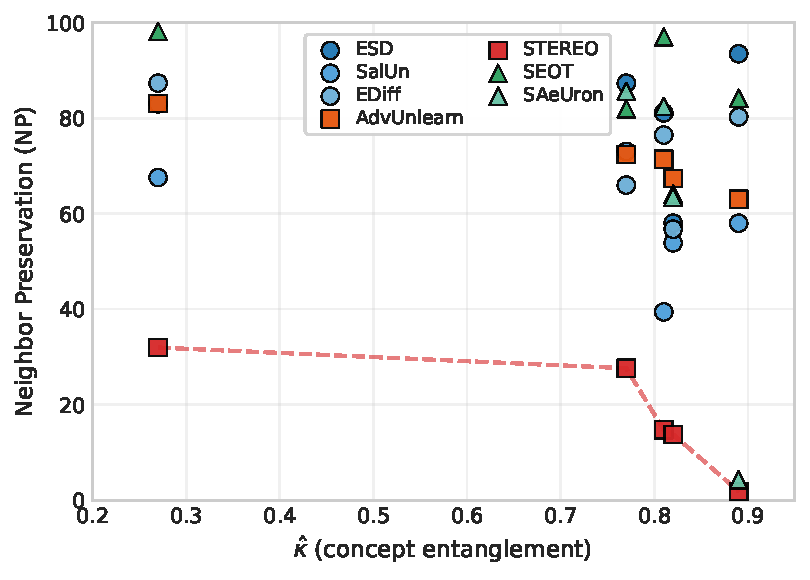
\includegraphics[width=\linewidth]{img/kappa_np_scaling.pdf}
\end{minipage}\hfill
\begin{minipage}[c]{0.45\linewidth}
\centering
\scriptsize
\setlength{\tabcolsep}{5pt}
\begin{tabular}{lccc}
\toprule
\textbf{Concept} & $\hat\kappa$ & NP$\uparrow$ & IRA-ratio$\uparrow$ \\
\midrule
\texttt{castle} & 0.27 & 31.96 & 0.55 \\
\texttt{cat}    & 0.77 & 27.60 & 0.32 \\
\texttt{horse}  & 0.81 & 14.71 & 0.29 \\
\texttt{bear}   & 0.82 & 13.75 & 0.25 \\
\texttt{dog}    & 0.89 & \phantom{0}1.81 & 0.06 \\
\midrule
\multicolumn{2}{l}{Spearman $\rho$} & $-1.0$ & $-1.0$ \\
\bottomrule
\end{tabular}
\end{minipage}
\caption{\textbf{Neighbor preservation scales inversely with $\hat\kappa$.} \emph{Left:} NP for each (method, concept) pair; STEREO's trend line (dashed) tracks $\hat\kappa$ monotonically. \emph{Right:} STEREO's NP and in-domain retention ratio across the five concepts (Spearman $\rho = -1.0$ for both).}
\label{fig:kappa_np_scaling}
\label{tab:kappa_scaling}
\vspace{-2mm}
\end{figure}



% \Cref{tab:kappa_scaling} reports STEREO's neighbor preservation (NP) and in-domain retention ratio, ordered by ascending $\hat\kappa$. Both decrease monotonically as $\hat\kappa$ increases: STEREO's NP drops from $31.96$ on \texttt{castle} to $1.81$ on \texttt{dog}, while its IRA-retention ratio drops from $59\%$ to $6\%$. The Spearman rank correlation with $\hat\kappa$ is $\rho = -1.0$ for both metrics across the five concepts, consistent with Eq.~\eqref{eq:tradeoff}.
% \begin{table}[t]
% \centering
% \setlength{\tabcolsep}{12pt}
% \begin{tabular}{lccc}
% \toprule
% \textbf{Concept} & $\hat\kappa$ & STEREO NP$\uparrow$ & IRA-ratio$\uparrow$ \\
% \midrule
% \texttt{castle} & 0.27 & 31.96 & 0.55 \\
% \texttt{cat}    & 0.77 & 27.60 & 0.32 \\
% \texttt{horse}  & 0.81 & 14.71 & 0.29 \\
% \texttt{bear}   & 0.82 & 13.75 & 0.25 \\
% \texttt{dog}    & 0.89 & \phantom{0}1.81 & 0.06 \\
% \midrule
% \multicolumn{2}{l}{Spearman $\rho$ vs. $\hat\kappa$} & $-1.0$ & $-1.0$ \\
% \bottomrule
% \end{tabular}
% \vspace{4pt}
% \caption{\textbf{$\hat\kappa$ predicts STEREO's trade-off severity.} STEREO's neighbor preservation (NP) and in-domain retention ratio (post-IRA / base-IRA) decrease monotonically with $\hat\kappa$ across the five target concepts. Both retention measures yield Spearman $\rho = -1.0$ rank-correlation with $\hat\kappa$, consistent with the linear $\kappa$-dependence in Eq.~\eqref{eq:tradeoff}.}
% \label{tab:kappa_scaling}
% \end{table}

\noindent{\bf The pattern generalizes beyond a single method.}
\Cref{fig:kappa_np_scaling} extends the analysis to all seven methods, plotting NP against $\hat\kappa$ for every (method, concept) pair. 
Three patterns are visible. First, robust fine-tuning methods (red and orange squares) exhibit the steepest $\hat\kappa$-dependence, with STEREO's NP (dashed trend line) tracking $\hat\kappa$ monotonically (Spearman $\rho = -1.0$) and AdvUnlearn similarly shows monotonic decrease. Second, inference-time methods (green triangles) show only weak $\hat\kappa$-dependence: their effective displacement $\Delta$ is too small for the $\kappa$-scaling in~\Cref{thm:tradeoff} to dominate, and NP remains near baseline regardless of concept. Third, standard fine-tuning methods (blue circles) occupy the middle band with intermediate $\hat\kappa$-sensitivity. This stratification reflects a structural principle: $\hat\kappa$ governs the structural lower bound on collateral damage, while the method's effective $\Delta$ determines how close it operates to that bound.
% \begin{figure}[t]
% \centering
% 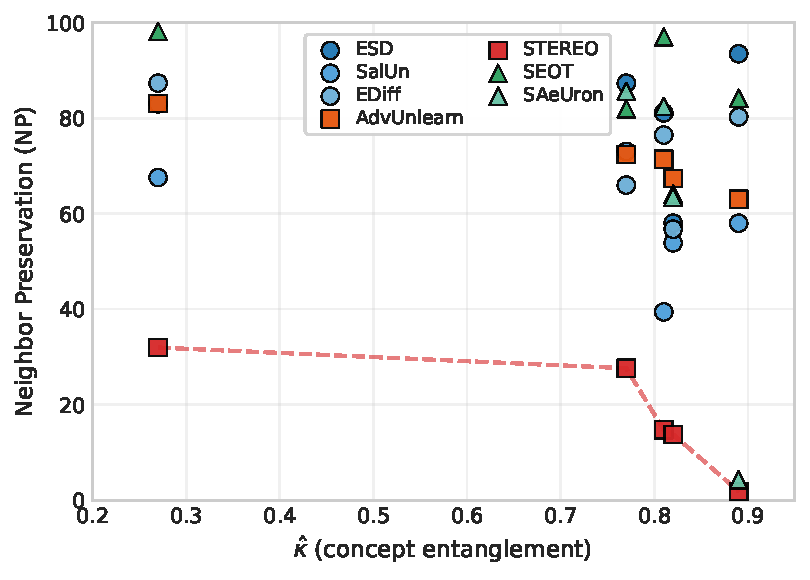
\includegraphics[width=0.5\linewidth]{img/kappa_np_scaling.pdf}
% \caption{\textbf{Neighbor preservation scales inversely with $\hat\kappa$ across methods.} Each point shows NP for one (method, concept) pair. Robust fine-tuning methods (red, square) exhibit the steepest $\hat\kappa$-dependence, with STEREO's NP (dashed trend line) tracking $\hat\kappa$ monotonically (Spearman $\rho = -1.0$). Inference-time methods (green, triangle) show weak $\hat\kappa$-dependence due to smaller effective displacement $\Delta$. Standard fine-tuning methods (blue, circle) lie in between. }
% \label{fig:kappa_np_scaling}
% \end{figure}
% \begin{figure}[t]
% \centering
% \begin{minipage}{0.48\linewidth}
%     \centering
%     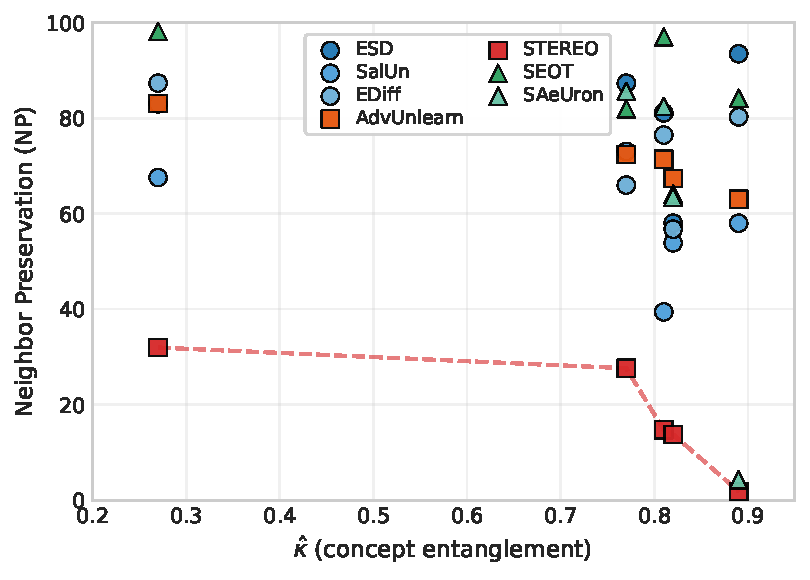
\includegraphics[width=\linewidth]{img/kappa_np_scaling.pdf}
% \end{minipage}
% \hfill
% \begin{minipage}{0.48\linewidth}
%     \caption{\textbf{Neighbor preservation scales inversely with $\hat\kappa$ across methods.}
%     Each point shows NP for one (method, concept) pair. Robust fine-tuning methods (red, square) exhibit the steepest $\hat\kappa$-dependence, with STEREO's NP (dashed trend line) tracking $\hat\kappa$ monotonically (Spearman $\rho = -1.0$). Inference-time methods (green, triangle) show weak $\hat\kappa$-dependence due to smaller effective displacement $\Delta$. Standard fine-tuning methods (blue, circle) lie in between.}
%     \label{fig:kappa_np_scaling}
% \end{minipage}
% \end{figure}

\noindent{\bf $\hat\kappa$ measures activation-space overlap, not semantic similarity.}
A natural concern is whether $\hat\kappa$ proxies for some other concept-level property such as semantic category (animal vs.\ architecture). Our estimator (\Cref{app:kappa_estimation}) is computed from sample-level overlap of activation regions, not from category labels or human-judged similarity. \texttt{Castle} ($\hat\kappa = 0.27$) and the four animal concepts ($\hat\kappa \in [0.77, 0.89]$) differ in $\hat\kappa$ not because they belong to different taxonomic categories but because castle's discovered neighbors 
% (\texttt{fortress}, \texttt{palace}, \texttt{citadel}) 
occupy sub-regions of activation space despite being semantically related, while animal subtypes 
% (e.g., \texttt{puppy}, \texttt{labrador} for \texttt{dog}; \texttt{mare}, \texttt{pony} for \texttt{horse}) 
densely overlap their target's region. 
The $\hat\kappa$ ordering is stable across probe layers (Spearman $\rho \geq 0.80$; \cref{app:layer_sensitivity}).
% The category label is descriptive; $\hat\kappa$ is the operative quantity \Cref{thm:tradeoff} predicts on, and the same procedure that yields $\hat\kappa = 0.27$ for \texttt{castle} yields $\hat\kappa = 0.89$ for \texttt{dog}.

% \noindent{\bf \Cref{thm:tradeoff} is a lower bound, not a ceiling.}
% \Cref{thm:tradeoff} bounds the \emph{minimum} collateral damage; methods may operate well above this minimum. STEREO on \texttt{castle} ($\hat\kappa = 0.27$) illustrates this: STEREO's DamageGap = $64.03$ is comparable to its damage on high-$\hat\kappa$ concepts despite the low predicted floor, while ESD (DamageGap = $6.77$) and SEOT (DamageGap = $0.79$) on the same concept achieve dramatically less damage. STEREO's REO objective broadly suppresses the spanned adversarial subspace regardless of neighbor proximity (\Cref{rem:stereo}), illustrating that $\kappa$-aware displacement remains an open direction for unlearning method design.

% \Cref{thm:tradeoff} predicts a $\kappa$-scaled \emph{minimum} on neighbor preservation error; it does not preclude methods from operating well above this minimum if their mechanism is mismatched to the concept's geometry. STEREO on \texttt{castle} illustrates this directly: despite the low predicted $\kappa$-floor, STEREO incurs DamageGap = $64.03$, comparable to its damage on the high-$\hat\kappa$ animal concepts. Other methods on \texttt{castle} achieve dramatically less collateral damage at similar erasure strength: ESD reaches NP = $83.03$ (DamageGap $= 6.77$) and SEOT reaches NP = $98.21$ (DamageGap $= 0.79$).
% This reflects the broad subspace suppression characteristic of STEREO's REO objective (\Cref{rem:stereo}), which displaces activations across the spanned adversarial directions regardless of whether neighbors actually occupy the displaced region. 
% A complementary indication of $\kappa$-blind suppression appears in STEREO's cross-domain preservation on \texttt{horse} (CP $= 27$, far below STEREO's CP on the other four concepts, range $64$--$96$): in the high-$\hat\kappa$ regime, STEREO's adversarial subspace spills beyond the intended object subspace into cross-domain features.
% The separation between STEREO and these alternatives on low-$\hat\kappa$ concepts suggests room for unlearning methods that achieve robust erasure with $\kappa$-aware rather than $\kappa$-blind displacement.



% \noindent{\bf Q3: Mechanism type determines the operating region.}
% Consistent with the mechanistic analysis in Remarks~\ref{rem:stereo}--\ref{rem:finetuning}, we observe a systematic separation between method families on the Pareto frontier:

% \begin{itemize}
%     \item \emph{Fine-tuning methods} modify model weights globally, displacing activations broadly across $\mathcal{R}_{c_u}$. They achieve stronger erasure (lower IRR) but incur more neighbor damage (lower NP). Among these, adversarially robust methods (STEREO, AdvUnlearn) push further toward the low-IRR / low-NP corner because their adversarial training explicitly targets the full extent of $\mathcal{R}_{c_u}$.
%     \item \emph{Inference-time methods} intervene on a narrow set of features or embeddings, producing smaller effective displacement $\Delta$. They preserve neighbors well (high NP) but leave portions of $\mathcal{R}_{c_u}$ unsuppressed, resulting in higher IRR. SAeUron, which blocks only $\tau_c$ sparse features, exemplifies this: it achieves the highest NP scores but is the most vulnerable to indirect concept recovery.
% \end{itemize}


\begin{comment}
    \subsection{Sequential Unlearning: Cumulative Collateral Damage}
\label{subsec:sequential}

A particularly revealing test of the trade-off is \emph{sequential unlearning}, where multiple concepts are erased from the same model in sequence. If concepts share representational structure, the collateral damage should accumulate: each additional erasure displaces more of the shared activation space, progressively degrading the model's retain performance.

We follow the sequential unlearning protocol of~\citet{zhang2024unlearncanvas} and~\citet{cywinski2025saeuron}, sequentially erasing up to 6 styles and measuring UA and RA ($= \frac{\mathrm{IRA} + \mathrm{CRA}}{2}$) after each step.

% TODO: Generate sequential unlearning results. Expected pattern:
% - Fine-tuning methods: RA drops steeply as more concepts are erased
% - SAeUron: RA remains stable (consistent with small per-concept Δ)
% - STEREO: RA drops most aggressively (consistent with large per-concept Δ)
% - Plot: line chart with number of erased concepts on x-axis, RA on y-axis, one line per method

\noindent The results confirm cumulative collateral damage for fine-tuning methods: RA degrades [progressively/sharply] as the number of erased concepts increases, consistent with the accumulating activation displacement predicted by our framework. SAeUron maintains stable RA throughout the sequence, consistent with its sparse, localized interventions producing minimal per-concept displacement. This experiment provides dynamic validation of the trade-off: it is not a one-time artifact but compounds with each additional unlearning step.

\end{comment}
